\section{Анализ существующих инструментов нагрузочного тестирования}

В условиях роста требований к надёжности веб-сервисов нагрузочное тестирование
стало неотъемлемой практикой в процессе разработки программного обеспечения.
Нагрузочное тестирование позволяет воспроизвести условия реальной эксплуатации,
выявить узкие места производительности и оценить поведение сервиса при пиковом
трафике ещё до развёртывания в промышленной среде~\cite{gost7322017}.
Без систематического проведения нагрузочных испытаний разработчики рискуют
обнаружить деградацию производительности уже в условиях промышленной эксплуатации,
когда стоимость устранения проблем многократно возрастает.

Существующие инструменты нагрузочного тестирования можно разделить на несколько
категорий: тяжёлые корпоративные решения с графическим интерфейсом,
скриптовые инструменты на базе JVM, лёгкие CLI-утилиты и облачные платформы.
Для обоснования разработки собственного инструмента был проведён сравнительный
анализ наиболее распространённых открытых решений.

\textbf{Apache JMeter}~--- один из старейших и наиболее функциональных инструментов
нагрузочного тестирования с открытым исходным кодом~\cite{jmeter}.
Распространяется в виде Java-приложения и требует наличия JVM версии~11 и выше.
JMeter поддерживает широкий спектр протоколов: HTTP, HTTPS, FTP, JDBC, LDAP и другие,
обладает развитым графическим интерфейсом для визуального конструирования
планов тестирования.
Вместе с тем инструмент отличается высокой сложностью настройки: конфигурация
хранится в XML-формате, а дистрибутив занимает более 60~МБ.
Потребление памяти JVM существенно ограничивает масштабируемость
на машинах с ограниченными ресурсами, а интеграция в конвейеры CI/CD требует
дополнительной настройки плагинов и сторонних инструментов разбора отчётов.

\textbf{Gatling}~--- высокопроизводительный инструмент нагрузочного тестирования,
ориентированный на HTTP-протокол~\cite{gatling}.
Написан на Scala и работает на платформе JVM, что влечёт те же зависимости
рантайма, что и Apache JMeter.
Сценарии тестирования описываются на предметно-ориентированном языке (DSL)
на основе Scala, что требует от пользователя базовых знаний этого языка.
Gatling генерирует подробные HTML-отчёты с перцентилями задержки и графиками
распределения, однако поддержка gRPC доступна только в коммерческой редакции
Gatling Enterprise.

\textbf{k6}~--- современный инструмент нагрузочного тестирования с открытым исходным
кодом, разработанный компанией Grafana Labs~\cite{k6}.
Бинарный файл написан на языке Go, однако сценарии нагрузочных тестов описываются
на JavaScript (TypeScript), что требует знания этого языка и усложняет автоматизацию
в простых сценариях.
k6 поддерживает HTTP, WebSocket и gRPC, предоставляет встроенную интеграцию с Grafana
Cloud для визуализации результатов.
Установка предполагает использование предкомпилированных бинарей или среды Node.js
при написании расширений.

\textbf{Vegeta}~--- минималистичный HTTP-инструмент нагрузочного тестирования,
написанный на языке Go~\cite{vegeta}.
Распространяется в виде единого бинарного файла без внешних зависимостей,
что делает его удобным для CI/CD-сред.
Vegeta поддерживает только протокол HTTP и не имеет встроенного веб-интерфейса
для мониторинга хода теста в реальном времени.
Конфигурация передаётся через стандартный ввод в текстовом формате,
что ограничивает сценарии использования динамически формируемыми нагрузками.

\textbf{hey}~--- простой HTTP-инструмент нагрузочного тестирования на Go,
ориентированный на быструю проверку производительности одного эндпоинта~\cite{hey}.
Не поддерживает gRPC, лишён веб-интерфейса и расширенных метрик ошибок;
результат выводится только в виде текстового отчёта по завершении теста,
что не позволяет отслеживать динамику метрик в ходе нагрузочного испытания.

Результаты сравнительного анализа представлены в таблице~\ref{tab:ch1-tools}.

\begin{table}[tbp]
  \centering
  \caption{Сравнительный анализ инструментов нагрузочного тестирования}
  \label{tab:ch1-tools}
  \small
  \begin{tabular}{@{}p{0.14\linewidth}p{0.13\linewidth}p{0.13\linewidth}p{0.12\linewidth}p{0.14\linewidth}p{0.18\linewidth}@{}}
    \toprule
    Инструмент     & Язык / рантайм & Протоколы      & Интерфейс & Зависимости       & Веб-интерфейс \\
    \midrule
    Apache JMeter  & Java (JVM)     & HTTP, gRPC, FTP & GUI, CLI  & JVM 11+           & Сторонние плагины \\
    Gatling        & Scala (JVM)    & HTTP            & CLI, HTML & JVM 11+           & HTML-отчёт (статика) \\
    k6             & Go + JS        & HTTP, WS, gRPC  & CLI       & Node.js (скрипты) & Grafana Cloud \\
    Vegeta         & Go             & HTTP            & CLI       & Нет               & Отсутствует \\
    hey            & Go             & HTTP            & CLI       & Нет               & Отсутствует \\
    \textbf{Tsunami} & \textbf{Go}  & \textbf{HTTP, gRPC} & \textbf{CLI + веб} & \textbf{Нет} & \textbf{Встроенный} \\
    \bottomrule
  \end{tabular}
\end{table}

Анализ таблицы~\ref{tab:ch1-tools} позволяет сделать следующие выводы.
Инструменты на базе JVM (JMeter, Gatling) обладают широким функционалом, однако
требуют наличия Java-рантайма и потребляют значительный объём оперативной памяти,
что затрудняет их использование в контейнерных и CI/CD-средах.
Инструменты на Go (Vegeta, hey) являются лёгкими и не имеют зависимостей,
однако ограничены только протоколом HTTP и не предоставляют визуального мониторинга.
k6 поддерживает gRPC и имеет интеграцию с Grafana, но для написания сценариев
требует знания JavaScript, а встроенная визуализация доступна только через
платный облачный сервис.

Таким образом, на рынке отсутствует инструмент, объединяющий лёгкость и
отсутствие зависимостей Go-бинаря, поддержку HTTP и gRPC в одном исполняемом файле
и встроенный веб-интерфейс с потоковой передачей метрик в реальном времени.
Данный пробел и определяет необходимость разработки инструмента Tsunami.


\section{Требования к разрабатываемому инструменту}

На основе проведённого анализа предметной области и выявленных недостатков
существующих решений были сформулированы требования к разрабатываемому
инструменту нагрузочного тестирования.

\textbf{Функциональные требования:}
\begin{enumerate}
  \item Поддержка нагрузочного тестирования HTTP-сервисов с настраиваемыми
    методом запроса, заголовками и телом.
  \item Поддержка нагрузочного тестирования gRPC-сервисов с возможностью
    указания .proto-файла или использования server reflection.
  \item Гибкое управление частотой запросов в формате \texttt{N/Vunit}
    (например, \texttt{100/1s}, \texttt{50/500ms}).
  \item Настройка числа параллельных воркеров и размера пула HTTP-соединений.
  \item Сбор и отображение метрик: общее число запросов, успехи, отказы,
    минимальная, средняя и максимальная задержка,
    перцентили p50, p95, p99, p99.9,
    пропускная способность (RPS), объём переданных данных.
  \item Классификация ошибок по типам: таймаут, отказ в соединении,
    ошибка DNS, ошибка TLS, прочие.
  \item Разбивка результатов по HTTP-кодам ответов.
  \item Веб-интерфейс для запуска тестов и визуализации метрик в реальном времени.
  \item REST~API для управления тестами из внешних систем (CI/CD).
  \item Экспорт результатов в формате JSON.
  \item Встроенная поддержка graceful shutdown по сигналам SIGINT/SIGTERM.
\end{enumerate}

\textbf{Нефункциональные требования:}
\begin{enumerate}
  \item Распространение в виде единого скомпилированного бинарного файла
    без внешних зависимостей рантайма.
  \item Кросс-платформенная поддержка: Linux, macOS, Windows;
    архитектуры amd64 и arm64.
  \item Корректная работа при целевой частоте не менее 1000~RPS
    при 50 параллельных воркерах на современном серверном оборудовании.
  \item Потокобезопасный сбор метрик без потери данных при высокой нагрузке.
  \item Задержка доставки метрик через WebSocket~--- не более 100~мс.
\end{enumerate}

Для наглядного представления вариантов использования системы была составлена
диаграмма прецедентов (рисунок~\ref{fig:ch1-usecase}), отражающая взаимодействие
двух категорий пользователей: CLI-пользователя и веб-пользователя.

\begin{figure}[tbp]
  \centering
  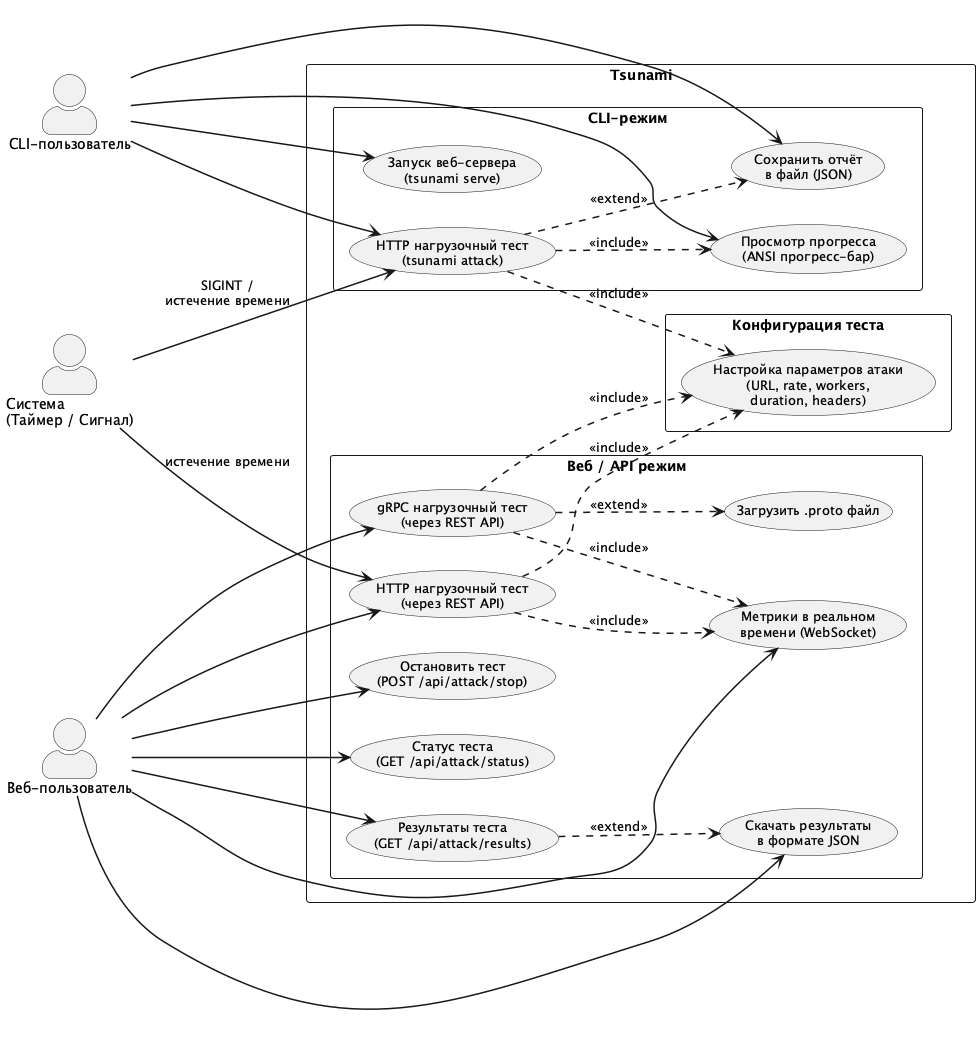
\includegraphics[width=0.92\linewidth]{assets/images/fig-01-tsunami-usecase.png}
  \caption{Диаграмма прецедентов системы Tsunami}
  \label{fig:ch1-usecase}
\end{figure}

CLI-пользователь взаимодействует с системой через команды \texttt{attack},
\texttt{serve} и \texttt{grpc}, получает живой прогресс в терминале
и сохраняет отчёт в файл.
Веб-пользователь управляет тестами через браузерный интерфейс,
получает метрики в реальном времени по протоколу WebSocket,
останавливает тест вручную и скачивает результаты.
Обе категории пользователей используют общий модуль конфигурации атаки.


\section{Выбор технологий и архитектурных решений}

Обоснованный выбор технологического стека является необходимым условием достижения
поставленных функциональных и нефункциональных требований.
В данном разделе приводится сравнительный анализ альтернатив и обоснование
принятых решений по каждому компоненту системы.

\subsection*{Язык программирования}

Для реализации ядра инструмента рассматривались три языка: Go, Python и Rust.

\textbf{Python} обладает развитой экосистемой для сетевого программирования
(asyncio, aiohttp), однако глобальная блокировка интерпретатора (GIL) ограничивает
параллельное выполнение CPU-нагрузки в нескольких потоках.
Кроме того, Python-приложение требует наличия интерпретатора на целевой машине,
что противоречит нефункциональному требованию о поставке единым бинарным файлом.

\textbf{Rust} обеспечивает наивысшую производительность и гарантии безопасности памяти
на уровне системы типов, однако обладает высоким порогом вхождения
и значительно увеличивает время разработки по сравнению с Go.

\textbf{Go} был выбран как оптимальный язык по совокупности характеристик~\cite{gospec}:
\begin{itemize}
  \item горутины~--- легковесные потоки исполнения с начальным размером стека ~2~КБ,
    позволяющие эффективно реализовать пул из сотен параллельных воркеров;
  \item встроенные примитивы конкурентности~--- каналы (\texttt{chan}),
    пакет \texttt{sync}, контексты (\texttt{context.Context})~---
    обеспечивают безопасную координацию горутин;
  \item статическая компиляция в единый бинарный файл без рантайм-зависимостей
    при установке флага \texttt{CGO\_ENABLED=0};
  \item богатая стандартная библиотека: \texttt{net/http} с пулом соединений,
    \texttt{crypto/tls}, \texttt{encoding/json};
  \item простая кросс-компиляция под любую целевую платформу через переменные окружения
    \texttt{GOOS} и \texttt{GOARCH}.
\end{itemize}

\subsection*{CLI-фреймворк}

Для организации интерфейса командной строки сравнивались библиотеки
\texttt{spf13/cobra} и \texttt{urfave/cli}.

\texttt{urfave/cli} предоставляет простой API, достаточный для однокомандных утилит,
однако слабо поддерживает вложенные субкоманды и не имеет встроенной
генерации документации.

\texttt{cobra}~--- стандарт де-факто для CLI-инструментов в экосистеме Go,
используется в таких проектах, как Docker, Kubernetes, Helm и GitHub CLI~\cite{cobra}.
Библиотека предоставляет гибкую систему субкоманд, автоматическую генерацию
справочного текста, поддержку персистентных флагов и хуки \texttt{PersistentPreRun}
для валидации входных параметров.
По результатам сравнения выбрана библиотека \texttt{cobra}.

\subsection*{Ограничение частоты запросов}

Для точного управления скоростью отправки запросов рассматривались три подхода:
\texttt{time.Ticker} из стандартной библиотеки, \texttt{golang.org/x/time/rate}
(алгоритм token bucket) и \texttt{go.uber.org/ratelimit} (алгоритм leaky bucket).

\texttt{time.Ticker} генерирует тики с фиксированным интервалом, однако при задержке
обработки тики накапливаются, что приводит к пиковым всплескам запросов
вместо равномерного потока.

\texttt{golang.org/x/time/rate} реализует token bucket: токены накапливаются
при простое и могут быть истрачены за один такт в режиме burst, что нежелательно
при воспроизводимом нагрузочном тестировании.

\texttt{go.uber.org/ratelimit} реализует алгоритм leaky bucket~\cite{ratelimit}:
метод \texttt{Take()} блокирует вызывающую горутину до момента, когда следующий
токен может быть выдан, обеспечивая строго равномерное распределение запросов
во времени.
Именно такое поведение критично для нагрузочного тестирования, где требуется
воспроизводимая постоянная нагрузка с заданным RPS.
Выбрана библиотека \texttt{go.uber.org/ratelimit}.

\subsection*{WebSocket}

Для реализации потоковой передачи метрик в реальном времени сравнивались
библиотеки \texttt{gorilla/websocket} и \texttt{nhooyr.io/websocket}.

\texttt{nhooyr.io/websocket}~--- более новая библиотека с контекстно-ориентированным API,
однако с меньшей зрелостью и значительно меньшим сообществом пользователей.

\texttt{gorilla/websocket}~--- наиболее широко применяемая Go-реализация протокола
WebSocket~\cite{gorilla}, используется в тысячах производственных проектов.
Библиотека обеспечивает полное соответствие RFC~6455, поддержку компрессии
и гибкую настройку параметров соединения.
По результатам сравнения выбрана \texttt{gorilla/websocket}.

\subsection*{Поддержка gRPC}

Поддержка gRPC реализована на основе официального Go-пакета
\texttt{google.golang.org/grpc}~\cite{grpcgo}~---
единственного зрелого gRPC-фреймворка для Go, поддерживаемого командой Google.
Для динамической компиляции .proto-файлов без использования внешнего компилятора
\texttt{protoc} применяется библиотека \texttt{bufbuild/protocompile},
предоставляющая программный интерфейс к компилятору Protocol Buffers.
Это позволяет пользователям передавать .proto-файлы непосредственно во время
выполнения теста без предварительной генерации кода.

\subsection*{Фронтенд}

Для разработки веб-интерфейса рассматривались три фреймворка: Angular, Vue.js и React.

\textbf{Angular}~--- полнофункциональный фреймворк с встроенными средствами управления
состоянием и строгой структурой проекта.
Для одностраничного дашборда мониторинга Angular является избыточным:
высокий порог вхождения и большой объём итогового бандла не соответствуют
требованию о встраивании фронтенда непосредственно в Go-бинарь.

\textbf{Vue.js}~--- прогрессивный фреймворк с простым API, однако экосистема библиотек
для визуализации данных в реальном времени уступает React-экосистеме по зрелости
и разнообразию компонентов.

\textbf{React}~18 в связке с TypeScript~5 был выбран как оптимальное решение~\cite{react}:
компонентный подход обеспечивает модульность, богатая экосистема предоставляет
готовые решения для всех задач, а строгая типизация TypeScript снижает
вероятность ошибок в рантайме.
Для визуализации метрик выбрана библиотека \textbf{Recharts}~---
декларативная SVG-библиотека графиков, органично интегрирующаяся с React.
Стилизация реализована с помощью \textbf{Tailwind CSS}, обеспечивающего
утилитарный подход к оформлению без необходимости писать отдельные CSS-файлы.

Встраивание скомпилированного React SPA в Go-бинарь выполнено с помощью
директивы \texttt{//go:embed}, что позволяет распространять единый исполняемый файл,
содержащий как серверную, так и клиентскую часть приложения~\cite{gospec}.

Итоговый технологический стек представлен в таблице~\ref{tab:ch1-stack}.

\begin{table}[tbp]
  \centering
  \caption{Технологический стек инструмента Tsunami}
  \label{tab:ch1-stack}
  \begin{tabular}{@{}p{0.22\linewidth}p{0.28\linewidth}p{0.42\linewidth}@{}}
    \toprule
    Компонент        & Технология                   & Обоснование выбора \\
    \midrule
    Язык бэкенда     & Go 1.25                      & Горутины, статический бинарь, кросс-компиляция \\
    CLI-фреймворк    & Cobra v1.10                  & Стандарт де-факто; субкоманды, хуки, генерация справки \\
    Rate limiting    & uber/ratelimit v0.3           & Leaky bucket; строго равномерный поток запросов \\
    WebSocket        & gorilla/websocket v1.5       & RFC~6455, зрелая библиотека, production-ready \\
    gRPC             & google.golang.org/grpc v1.80 & Официальный Go gRPC-фреймворк от Google \\
    Компилятор proto & bufbuild/protocompile v0.14  & Динамическая компиляция .proto без protoc \\
    UI-фреймворк     & React 18 + TypeScript 5      & Компонентность, экосистема, типобезопасность \\
    Графики          & Recharts 2.10                & Декларативные SVG-графики, интеграция с React \\
    CSS-фреймворк    & Tailwind CSS 3.4             & Утилитарный подход, малый итоговый бандл \\
    Встраивание SPA  & go:embed                     & Единый бинарь без внешних статических файлов \\
    Сборщик          & Vite 5                       & Быстрая сборка, нативная поддержка TypeScript \\
    \bottomrule
  \end{tabular}
\end{table}


\section{Проектирование архитектуры системы}

На основе сформулированных требований и выбранного технологического стека была
спроектирована трёхслойная архитектура инструмента Tsunami.

\subsection*{Компонентная структура}

Система состоит из трёх основных слоёв.

\textbf{CLI-слой} (\texttt{cmd/}) реализован на основе фреймворка Cobra и включает
три субкоманды: \texttt{attack} (HTTP-тестирование), \texttt{grpc}
(gRPC-тестирование) и \texttt{serve} (запуск веб-сервера).
Слой отвечает за парсинг флагов командной строки, валидацию входных параметров
и вывод результатов в терминал или файл.

\textbf{Движок нагрузочного тестирования} (\texttt{internal/attack/},
\texttt{internal/grpcattack/}) является ядром системы.
Содержит конфигурационные структуры (\texttt{AttackConfig}), пул воркеров,
диспетчер задач с ограничением скорости, потокобезопасный сборщик метрик
(\texttt{GlobalMetrics}) и генератор JSON-отчётов.

\textbf{HTTP-сервер с веб-интерфейсом} (\texttt{cmd/server/}) предоставляет
REST~API для управления тестами, WebSocket-хаб для стриминга метрик
и встроенное React-приложение.

Принципиально важным архитектурным решением является то, что CLI-слой
и HTTP-сервер используют один и тот же движок нагрузочного тестирования.
Это исключает дублирование бизнес-логики и гарантирует идентичное поведение
системы вне зависимости от способа управления~--- через терминал или браузер.

\subsection*{Паттерн «пул воркеров»}

Движок нагрузочного тестирования построен на паттерне «пул воркеров»
с каналами задач и результатов (рисунок~\ref{fig:ch1-workerpool}).

\begin{figure}[tbp]
  \centering
  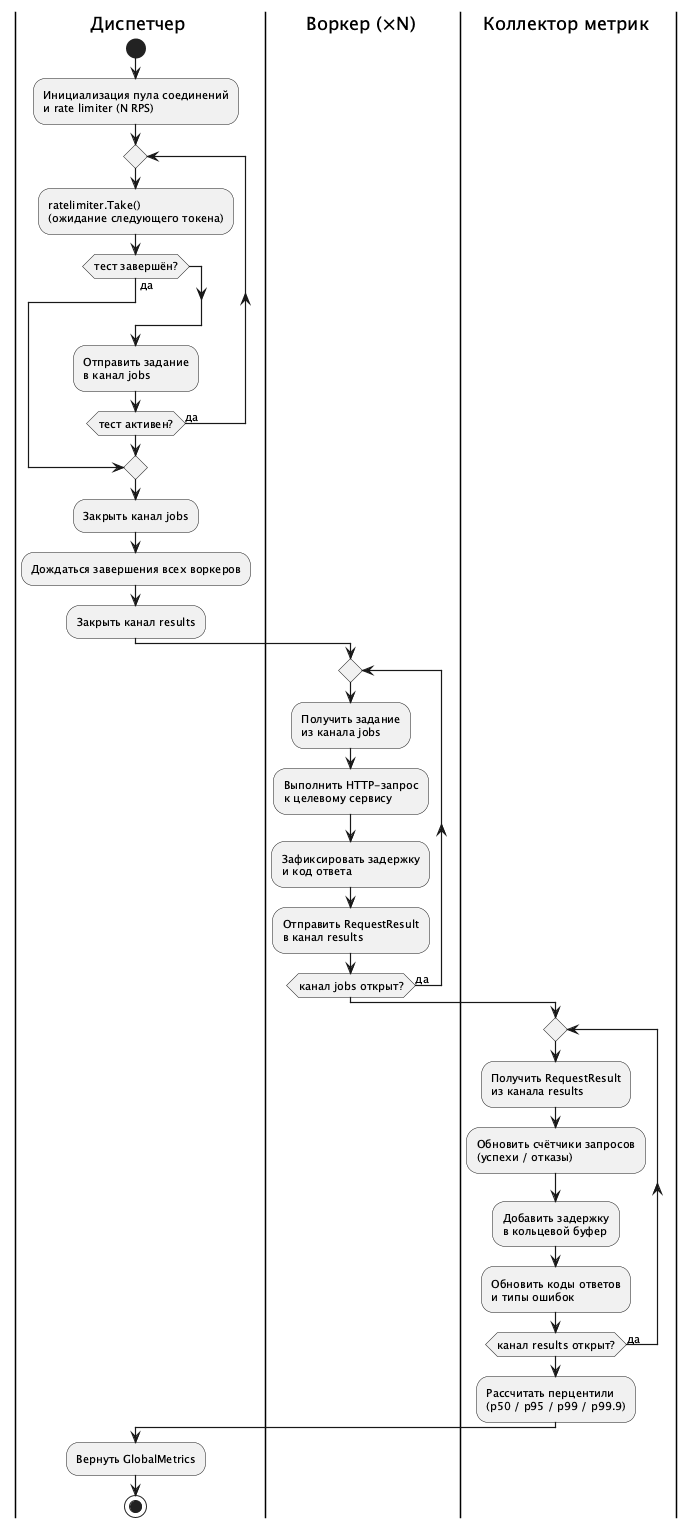
\includegraphics[width=\linewidth,height=0.72\textheight,keepaspectratio]{assets/images/fig-02-tsunami-workerpool.png}
  \caption{Схема взаимодействия компонентов движка нагрузочного тестирования}
  \label{fig:ch1-workerpool}
\end{figure}

Диспетчер задач в цикле вызывает метод \texttt{ratelimiter.Take()},
который блокирует выполнение до наступления следующего разрешённого момента
согласно алгоритму leaky bucket.
После получения токена диспетчер помещает задание в буферизованный канал \texttt{jobs}.

$N$ горутин-воркеров одновременно ожидают заданий из канала \texttt{jobs}.
Получив задание, каждый воркер выполняет HTTP- или gRPC-запрос к целевому сервису,
фиксирует время ответа и помещает объект \texttt{RequestResult} в канал \texttt{results}.
Структура \texttt{RequestResult} содержит код ответа, задержку, признак успеха,
тип ошибки и объём переданных данных.

Горутина-коллектор последовательно считывает результаты из канала \texttt{results}
и накапливает их в структуре \texttt{GlobalMetrics}, защищённой мьютексом.
Такое разделение ответственности позволяет воркерам не блокироваться на операциях
агрегации метрик и достигать высокой пропускной способности.

\subsection*{Структура GlobalMetrics и расчёт перцентилей}

Структура \texttt{GlobalMetrics} обеспечивает потокобезопасный сбор всех метрик теста.
Для хранения значений задержки используется кольцевой буфер
(\texttt{Latencies []time.Duration}) ёмкостью 100\,000~элементов.
При каждом добавлении нового значения индекс сдвигается по модулю размера буфера,
что гарантирует ограниченное потребление оперативной памяти
вне зависимости от длительности теста и числа запросов.

Перцентили задержки (p50, p95, p99, p99.9) вычисляются по завершении теста
функцией \texttt{CalculateAllPercentiles}: буфер сортируется однократно,
после чего значения перцентилей считываются из соответствующих позиций
отсортированного массива.
Однократная сортировка вместо четырёх независимых вызовов снижает вычислительную
сложность с $O(4 \cdot n \log n)$ до $O(n \log n)$.

Для построения временного графика задержки используется отдельный буфер
\texttt{LatencyHistory} ёмкостью 1\,000~точек: сэмплирование выполняется
каждые~10 запросов, что обеспечивает равномерное покрытие всего интервала теста
вне зависимости от его продолжительности.

\subsection*{Конечный автомат TestSession}

При управлении тестом через веб-интерфейс жизненный цикл каждого испытания
контролируется объектом \texttt{TestSession}, реализующим конечный автомат
с пятью состояниями (рисунок~\ref{fig:ch1-statemachine}).

\begin{figure}[tbp]
  \centering
  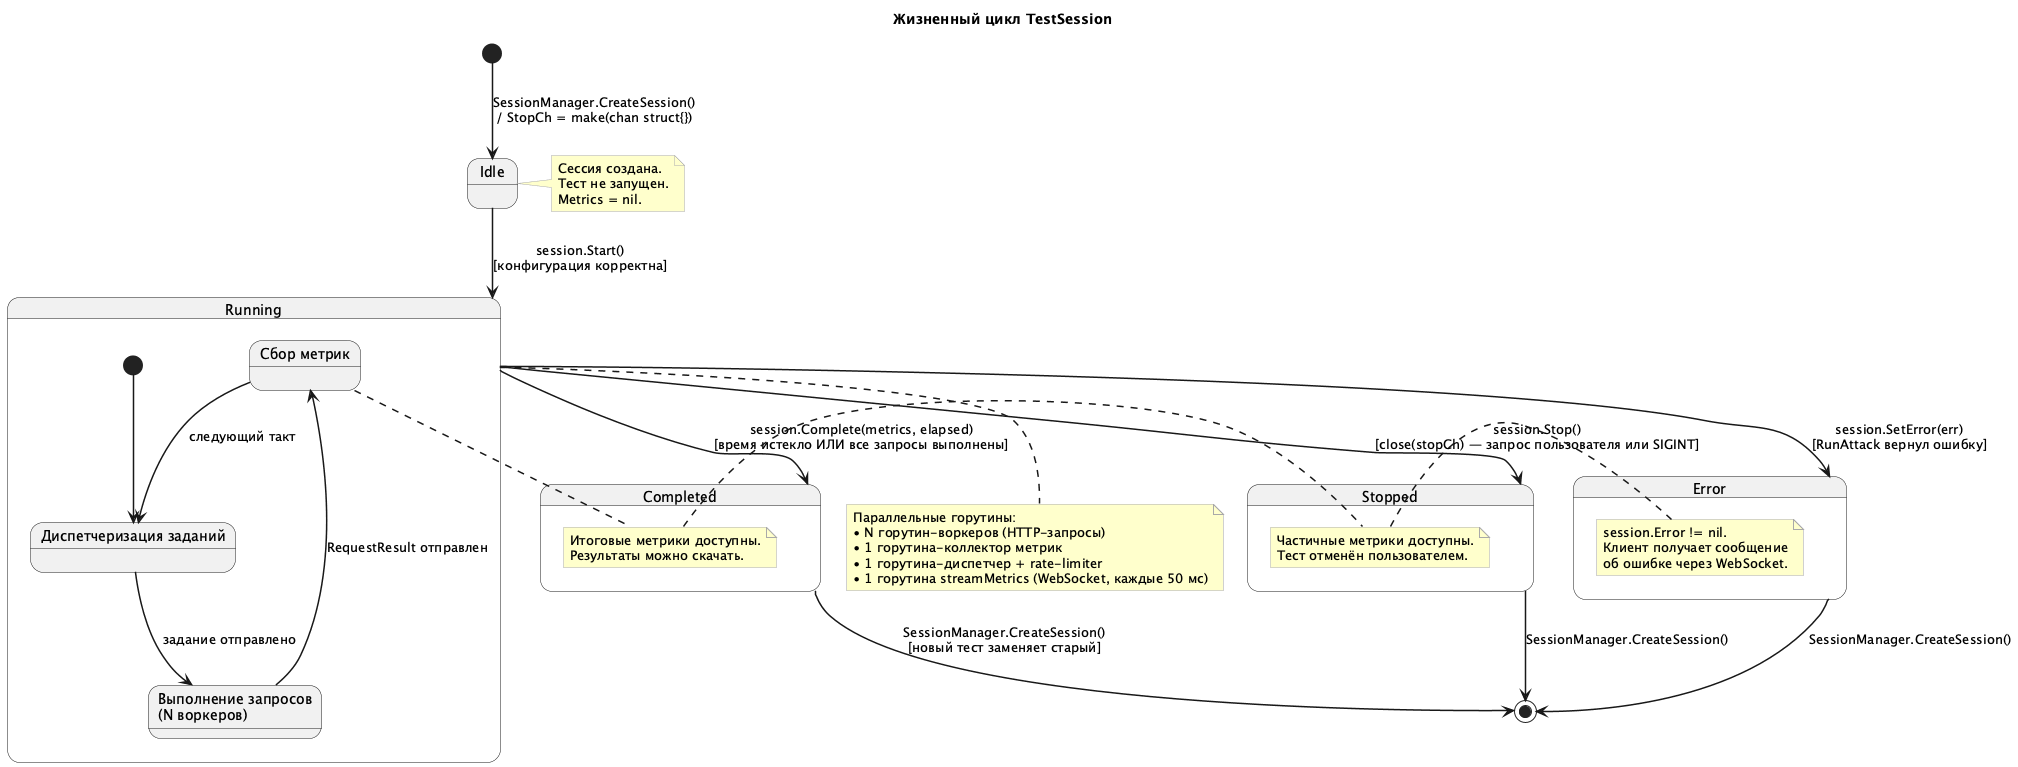
\includegraphics[width=0.80\linewidth]{assets/images/fig-03-tsunami-statemachine.png}
  \caption{Диаграмма состояний объекта TestSession}
  \label{fig:ch1-statemachine}
\end{figure}

В состоянии \textbf{Idle} сессия создана, но тест ещё не запущен.
Переход в состояние \textbf{Running} происходит при вызове метода
\texttt{session.Start()}.
Из состояния Running возможны три перехода:
в \textbf{Completed}~--- по истечении заданной длительности теста;
в \textbf{Stopped}~--- при явной остановке пользователем через REST~API;
в \textbf{Error}~--- при возникновении критической ошибки в движке атаки.

Остановка теста реализована через канал \texttt{StopCh} типа \texttt{chan struct{}}.
Закрытие канала является неблокирующим широковещательным сигналом для всех горутин,
которые отслеживают его состояние через конструкцию \texttt{select}.

\subsection*{WebSocket-хаб и стриминг метрик}

Для трансляции метрик подключённым браузерным клиентам применяется
паттерн «хаб» (\texttt{Hub}).
Хаб поддерживает три канала: \texttt{register}, \texttt{unregister} и \texttt{broadcast}.
Горутина \texttt{Hub.Run()} в цикле обрабатывает эти каналы:
регистрирует новых клиентов, удаляет отключившихся и рассылает сообщения
всем активным соединениям.

Отдельная горутина \texttt{streamMetrics} с интервалом 50~мс считывает текущее
состояние \texttt{GlobalMetrics}, формирует объект \texttt{MetricsPayload}
и передаёт его в канал \texttt{broadcast} хаба.
Каждый клиент имеет собственный буферизованный канал \texttt{send} ёмкостью
256~сообщений и отдельные горутины \texttt{readPump}/\texttt{writePump},
что предотвращает блокировку хаба при наличии медленных или зависших клиентов.

\subsection*{REST API сервера}

HTTP-сервер предоставляет следующие эндпоинты (таблица~\ref{tab:ch1-api}):

\begin{table}[tbp]
  \centering
  \caption{Эндпоинты REST API инструмента Tsunami}
  \label{tab:ch1-api}
  \begin{tabular}{@{}p{0.10\linewidth}p{0.34\linewidth}p{0.48\linewidth}@{}}
    \toprule
    Метод & Путь & Описание \\
    \midrule
    POST & \texttt{/api/attack/start}            & Запуск нагрузочного теста \\
    POST & \texttt{/api/attack/stop}             & Остановка текущего теста \\
    GET  & \texttt{/api/attack/status}           & Текущий статус и метрики теста \\
    GET  & \texttt{/api/attack/results}          & Итоговые результаты после завершения \\
    GET  & \texttt{/api/attack/results/download} & Скачать результаты в формате JSON \\
    POST & \texttt{/api/proto/upload}            & Загрузить .proto-файл для gRPC \\
    WS   & \texttt{/ws/metrics}                  & WebSocket: стриминг метрик (50~мс) \\
    GET  & \texttt{/health}                      & Проверка работоспособности сервера \\
    \bottomrule
  \end{tabular}
\end{table}

Маршрутизация организована таким образом, что все запросы к путям \texttt{/api/},
\texttt{/ws/} и \texttt{/health} обрабатываются API-мультиплексором,
а все остальные пути передаются обработчику SPA (\texttt{SPAHandler}),
который возвращает \texttt{index.html} для поддержки клиентской маршрутизации React.
К серверу применяется CORS-middleware, разрешающий кросс-доменные запросы
в режиме разработки.

Таким образом, спроектированная архитектура обеспечивает чёткое разделение
ответственности между слоями: CLI и веб-сервер используют единый движок
нагрузочного тестирования, что исключает дублирование бизнес-логики.
Применение паттернов пула воркеров, конечного автомата и WebSocket-хаба
позволяет достичь высокой производительности и удобства мониторинга в реальном времени.
Принятые в данной главе архитектурные решения реализуются в главе~2.
